

\afterpage{\null\newpage}
\chapter{Adaptive Sampling Comparison\label{ch:chapter32}}

One major challenge in developing, investigating and comparing adaptive sampling strategies are the large computational resources required to run adaptive sampling with the necessary molecular dynamics trajectories. To reach statistically significant sample sizes requires even larger computational resources which are rarely available.
The investigation of adaptive sampling for toy systems or small peptides requires lower amount of computational resources. The lower dimensionality of these smaller test systems reduces the transferability of the resulting conclusions to biomolecules which have an order of magnitude more degrees of freedom and a more complex energy landscape. Some strategies which work well for toy systems of small peptides face significant challenges to scale up to larger proteins. 
An alternative approach to investigating adaptive sampling strategies for larger biomolecules is the utilization of Markov Chain trajectories. These approximations of molecular dynamics trajectories can be generated many orders of magnitudes faster than molecular dynamics trajectories, allowing a better sample size than generating molecular dynamics trajectories for adaptive sampling. The requirement for the generation of Markov Chain trajectories is the knowledge of the Markov State Model of a protein.  In this chapter adaptive sampling strategies are investigated with Markov Chain trajectories, the material in this chapter was first published in: 

\cite{Adstrategies2018} \textbf{Hruska, E.}; Abella, J. R.; N\"uske, F.;
Kavraki, L. E. \& Clementi, C.; Quantitative
comparison of adaptive sampling methods
for protein dynamics. J. Chem. Phys. 149 (2018) 



\section{\label{sec:methods}Methods}


\subsection{\label{sec:methods-dataset}Reference Dataset of Simulations}

To generate accurate Markov State Models which well sampled simulations are necessary. Here we used published long all-atom molecular dynamics trajectories from Anton supercomputer\cite{lindorff2011}.
The Table\ref{tab:dataset-summary} shows the 8 proteins utilized. The 8 proteins are ranging  from 10 to 80 residues. These proteins have with different topologies, both $\alpha$-helices, $\beta$ sheets and a  mix of both. The folding times in simulation are ranging from $0.6$ to $49$ $\mu$s. These protein are relaltively fast folding since only fast folding proteins can be currently simulation with multiple folding and unfolding events.

\begin{table}[!ht]
\centering
\caption{Proteins for reference data}
\label{tab:dataset-summary}
\resizebox{\columnwidth}{!}{
\begin{tabular}{|c|c|c|c|c|c|}
\hline
Protein Name & PDB ID of Folded Structure & Size (\# residues) & Folding Time ($\mu$s) from \cite{lindorff2011}\\ 
\hline
Chignolin    & 2RVD                       & 10                 & 0.6                 \\
Trp-cage     & 2JOF                       & 20                 & 14                  \\
BBA          & 1FME                       & 28                 & 18                  \\
WW Domain    & 2F21                       & 35                 & 21                 \\
Protein B    & 1PRB                       & 47                 & 3.9                  \\
Homeodomain  & 2P6J                       & 52                 & 3.1                  \\
$\alpha$3D   & 2A3D                       & 73                 & 27                  \\
$\lambda$-repressor  & 1LMB               & 80                 & 49             \\ 
\hline            
\end{tabular}
}
\end{table}

\subsection{\label{sec:methods-msm}Construction of Markov State Models}

Markov Chain trajectories can approximate molecular dynamics trajectories only when the Markov State Models are accurate. The MSM respresents the biomolecules stationary and dynamic behavior. 
We have used the standard procedures to generate MSM. The trajectories were dimension-reduced with Time-lagged Independent Component Analysis (TICA) 
\cite{TICA1-perez2013, TICA2-schwantes2013}, where the output dimension are scaled according to commute map 
\cite{noe2016commute}. The input features for TICA were all pairwise
inter-residue distances and all dihedral angles of the protein.  The pairwise
inter-residue distance is the closest heavy-atom distance between a pair of residues. 
For the smaller proteins,  additional features of inverse inter-residue distances were used to increase the accuracy. This dimensional reduced space was clustered with k-means clustering into 1000 or 2000 states, depending on the size and sampling of the protein. This larger number of microstates is selected to increase accuracy of the Markov Chain trajectories and is only possible due to the good sampling of the reference trajectories. The disconnected microstates were removed and the folding-unfolding process was set as the slowest MSM eigenvector. 

For each protein, a set of folded and unfolded states are defined. The native contacts are extracted from the folded structures shown in Table \ref{tab:dataset-summary}. For each state, the median number of native
contacts is determined. States with median number of native contacts above a folding threshold are assigned as the folded states. States with native contacts above a unfolding threshold are set as the unfolded states.

The clustering results in microstate trajectories. The reference MSMs are generated by maximum-likelihood estimation under detailed balance
constraint. The lag time $\tau$ for MSM generation was selected based on the plateau of implied timescales. The Markov property of the resulting MSM was tested by Chapman-Kolmogorov validation. All this
analysis was executed with the PyEMMA package \cite{scherer2015pyemma}. Details of the MSM generation are described in the paper\cite{Adstrategies2018}.To generate Markov Chain trajectories, synthetic microstate trajectories are generated according to the transition probabilities of the MSM transition matrix.

 

\subsection{\label{sec:level5}Simulating adaptive sampling with Markov Chain trajectories}

The simulation of adaptive sampling with Markov Chain trajectories follows the schematic in Chapter 3 Figure~\ref{fig:schema2}. 
Instead of simulating an ensemble of $n$ MD trajectories and ensemble of $n$ Markov Chain trajectories is simulated. The required time for simulating Markov Chain trajectories is order of magnitudes smaller than simulating equivalent MD trajectories. This allows to simulate many repetitions of adaptive sampling and for multiple proteins.

The investigated sampling strategies are plain MD as reference, and $cmicro$, the 4 $cmacro$ strategy variants, the two adaptive sampling strategies with \emph{a priori} information $Q_{f}$ and $Q_{f,nn}$ and the two optimal strategies for adaptive sampling performance $p_{esc}$ and $t_{opt}$.  These strategies were described in Chapter 3.
At the end of each iteration of each strategy a new set of $n$ restarting points are chosen. The restarting points were chosen based on the adaptively sampled MSM. This iteratively updating adaptively sampled MSM represents only the explored transitions captured in the sampled Markov Chain trajectories. 

Two of the $cmacro$ strategy variants include the Koopman method to improve the accuracy of the Markov State model. The Koopman method applies directly to the molecular dynamics trajectory which is not available here. To estimated the effect of the Koopman methods on adaptive sampling, the adaptively sampled MSM is corrected to the transition probabilities from the reference MSMs. This approach gives an upper limit on the improvement of adaptive sampling the Koopman method can achieve. 


\section{\label{sec:results}Results}

Once the adaptive sampling is generated for each protein, each sampling strategy and repeated 100 times, the sampling can be evaluated according to different sampling objectives.
Here we quantify the adaptive sampling performance by two sampling objectives. The first objective is the time to cross the rare transition barrier or folding of the protein. The second objective is the time to explore 95\% of the states, representing the exploration of the whole energy landscape.
In each case the average and the 20\% and 80\% percentiles are measured and compared with the other sampling strategies, including plain MD.  
In each case a parallelization $n$ of 100 replicas is chosen, except for the scaling comparison where the parallelization $n$ ranges from 1 to 5000. 

\subsection{\label{sec:time-fold}Time to fold}

\begin{figure}[H]
  %%\centering
  \begin{subfigure}[t]{0.5\textwidth}
    \includegraphics[width=0.9\textwidth]{figures/CLN025_7_steps10000_nparallel100_fold.eps} 
  \end{subfigure}
  \begin{subfigure}[t]{0.5\textwidth}
    \includegraphics[width=0.9\textwidth]{figures/GTT_7_steps10000_nparallel100_fold.eps}  
  \end{subfigure}
  \begin{subfigure}[t]{0.5\textwidth}
    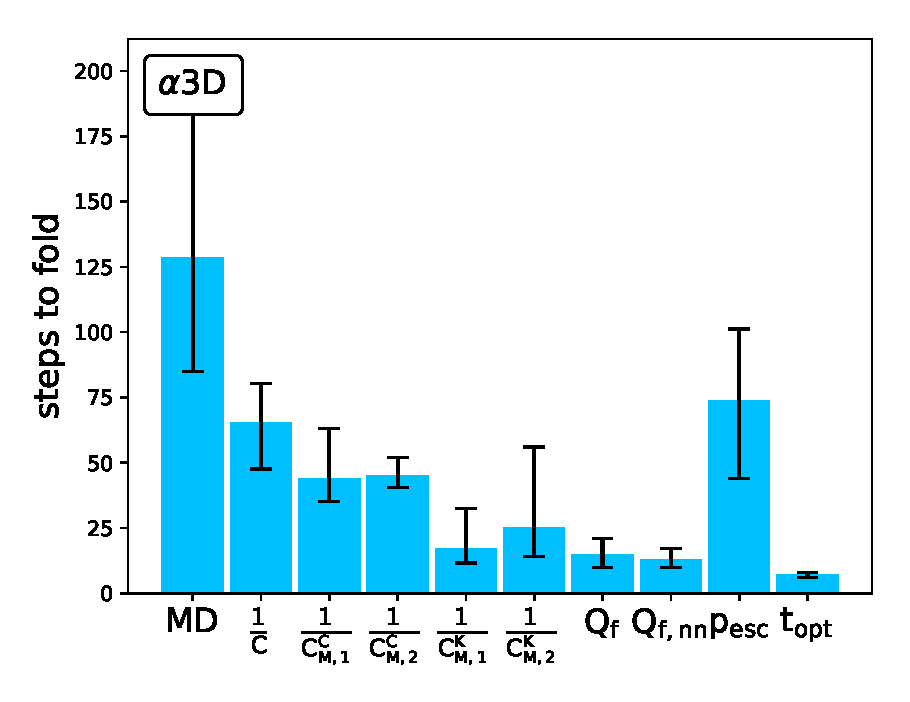
\includegraphics[width=0.9\textwidth]{figures/A3D_7_steps10000_nparallel100_fold.eps}   
  \end{subfigure}
  \caption{Time to fold for the different sampling strategies for proteins Chignolin, WW Domain and $\alpha$3D.}
  \label{fig:Time_fold}
\end{figure}


The time to folding of the protein is the most common objective of adaptive sampling. Figure~\ref{fig:Time_fold} shows the performance of different adaptive sampling strategie with Markov Chain trajectories.
Each sampling strategy should be compared with plain MD which is the reference sampling strategy.
The simple $cmicro$/$1/C$ strategy shows no speed up for Chignolin, WW Domain and only a small 2x speed up for $\alpha$3D. This shows that the $cmicro$ strategy is not optimal for folding proteins. The reason for the low efficiency lies in the oversampling of states which are not on the folding path, but have a low stationary probability and high restart probability.

The $cmacro$ strategies show a significant speed up compared to plain MD for all the proteins, but the 4 variants of the $cmacro$ strategies show significant performance differences.
Between the 4 variants of the $cmacro$ strategies it seems the the correction of the MSM due to non-equilibrium  $1/C_{K, 1}$ improves the results most. While the approximation of the Koopman method with the Markov Chain trajectories is only a upper limit for the performance improvement, the improvement is 2-3x. The improved performance of the corrected MSMs is caused by the improved estimation of the collective motions of the proteins. The estimated macrostates are kinetically more accurate. The 2 variants in setting the number of macrostates doesn't show a large performance effect. The constant number
of macrostates $1/C_{M, 1}$ is slightly faster. The underperformance of the kinetically set number of macrostates could be cause by the challenge to accurately determine the timescales for partially sampled energy landscapes.

The two adaptive sampling strategies with \emph{a priori} information $Q_{f}$ and $Q_{f,nn}$ show significant improvement over $1/C_{K, 1}$, which is the best strategy without \emph{a priori} information. If the \emph{a priori} information is accurate then this can speed up the folding of the protein significantly. Depending on the protein the improvement with the \emph{a priori} information can be less than 50
\% or a factor 2-3x. The effectivity of including dimension of \emph{a priori} information to prevent misfolded states in  $Q_{f,nn}$ varies on the protein, but no significant performance penalties are observed.

The two benchmark strategies $p_{esc}$ and $t_{opt}$ show very different performance. The strategy optimized to fold proteins $t_{opt}$  shows the upper limit for protein folding speed up with adaptive sampling. This benchmark shows an 2x or more improvement compared to strategies with no \emph{a priori} information, allowing a gap for the improvement of adaptive sampling strategies. Previously the upper limit for performance of protein folding with adaptive sampling was unknown. The $t_{opt}$ strategy is in some proteins close to the performance of $Q_{f,nn}$, the best strategy with \emph{a priori} information. The similar performance can be cause due to the simple protein folding pathway. For other proteins the $t_{opt}$ strategy is significantly faster than $Q_{f,nn}$, showing that adaptive sampling strategies with \emph{a priori} information have opportunities to improve. The strategy optimized to explore all states undiscrimatedly $p_{esc}$ isn't effective in folding proteins. The performance of the adaptive sampling strategies is consistent between different protein, allowing to conclude that adaptive sampling is effective for different topologies, both $\alpha$-helices and $\beta$ sheets.

\subsection{\label{sec:time-explore}Time to explore 95\% of states}

\begin{figure}[H]
  %%\centering
  \begin{subfigure}[t]{0.5\textwidth}
    \includegraphics[width=0.9\textwidth]{figures/CLN025_7_steps10000_nparallel100_explore.eps}
  \end{subfigure}
  \begin{subfigure}[t]{0.5\textwidth}
    \includegraphics[width=0.9\textwidth]{figures/1FME_7_steps10000_nparallel100_explore.eps}   
  \end{subfigure}
  \begin{subfigure}[t]{0.5\textwidth}
    \includegraphics[width=0.9\textwidth]{figures/A3D_7_steps10000_nparallel100_explore.eps}   
  \end{subfigure}
  \caption{Time to the exploration of 95\% of the states for the different sampling strategies for proteins Chignolin, BBA and $\alpha$3D.}
  \label{fig:Time_explore}
\end{figure}

Figure~\ref{fig:Time_explore} shows the average time needed for the different
adaptive sampling strategies to explore 95\% of the microstates constituting the
MSM, by using 100 parallel trajectories, for three different proteins.
In this comparison we exclude the strategies designed to speedup the sampling
of the folding process (such as the native contact based strategies as well as
$t_{opt}$) because they are not designed for the purpose of general exploration.
The comparison shows that, in general, the $1/C$ strategy explores the
configurational space much more efficiently than plain MD. The speedup obtained
by the $1/C$ strategy nears the theoretical maximum obtained by the optimal
exploration strategy, $p_{esc}$. Within the macrostate-based strategies, there
is more variance. The strategies using the regular count matrix $(1/C_M^C)$ outperform
the strategies that correct for non-equilibrium errors, $(1/C_M^K)$. This is
likely because the correction introduces a bias towards the sampling of slow
processes rather than general exploration. The non-equilibrium error in the
count matrix based strategies introduces randomness that helps the sampling of
unexplored microstates. Additionally, for some proteins the optimization of the number of
macrostates based on the kinetic content ($1/C_{M, 2}$) does appear to provide
an advantage over the use of a constant number of macrostates ($1/C_{M, 1}$). 
The use of the kinetic content allows for a more accurate estimation of
macrostate counts, which could help to focus the sampling bias towards regions
that are less densely sampled. 
The patterns shown in Fig.~\ref{fig:Time_explore}
are consistent across all the proteins and across the number of
parallel trajectories used. The corresponding plots for all the proteins can be
found in the Supplementary material.

\subsection{\label{sec:scaling}Scaling}

\begin{figure}[H]
  %%\centering
  \begin{subfigure}[t]{0.5\textwidth}
    \includegraphics[width=0.9\textwidth]{figures/GTT_6_steps10000_scaling_fold0.eps}    
  \end{subfigure}
  \begin{subfigure}[t]{0.5\textwidth}
    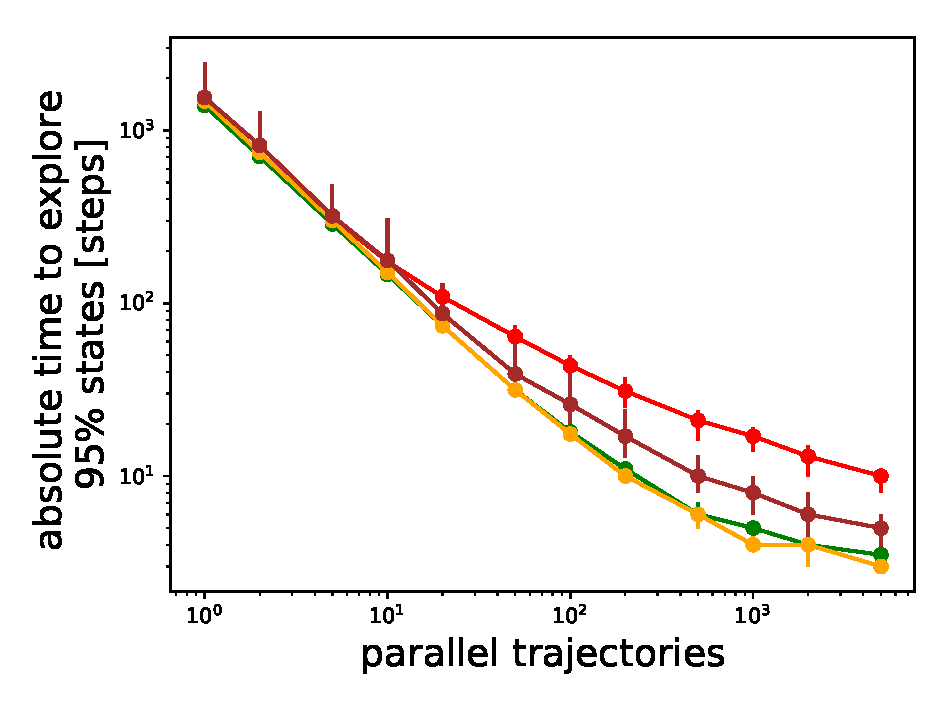
\includegraphics[width=0.9\textwidth]{figures/1FME_6_steps10000_scaling_explore.eps}
    %%\caption{$\lambda$-repressor}    
  \end{subfigure}
  \begin{subfigure}[t]{0.5\textwidth}
    \includegraphics[width=0.9\textwidth]{figures/1FME_6_steps10000_scaling_explore_total.eps}
    %%\caption{$\lambda$-repressor}    
  \end{subfigure}
  \caption{Top: Scaling of the absolute folding time required to fold the
  protein model for the WW Domain for 5 different sampling strategies: plain
  $MD$, $p_{esc}$, $t_{opt}$, $1/C$ and $1/C_{M,2}^K$. Scaling of the
  absolute (middle) or cumulative (bottom) number of steps required to explore
  95\% of all microstates, for the protein  model of BBA, for 3 different
  strategies: plain $MD$, $p_{esc}$, $1/C$ and $1/C_{M,2}^K$.  
  The 20\% and 80\% percentiles are shown as error bars. 
  Similar figures for the other
  protein models are reported in the Supplementary material.}
  \label{fig:scaling}
\end{figure}

Adaptive sampling methods capitalize on the use of many relatively short
parallel trajectories, usually deployed on massively parallel computers (MPC),
to speed up rare events or explore protein conformational spaces. In order to
better understand the limits of scalability of adaptive sampling strategies,
the measured absolute folding time for different parallelization is shown in
Figure \ref{fig:scaling}. The absolute folding time indicates the actual clock
time required to record a folding event for a given protein on MPC with a given
adaptive sampling strategy. The different strategies exhibit good scaling below
a parallelization of around 100 and moderate scalability up to 1000 parallel
trajectories. The scalability differs only slightly between different
strategies, confirming that adaptive sampling generally scales well.
Similar scaling is observed for all protein models. The time to explore 95\% of
microstates in Figure \ref{fig:scaling} scales to a higher parallelization than
the time to fold the protein. In addition to Fig.
\ref{fig:scaling}, scaling plots for the other protein models are
available in the Supplementary material. 

\begin{figure}[H]
  %%\centering
  \begin{subfigure}[t]{0.5\textwidth}
    \includegraphics[width=0.9\textwidth]{figures/compare_MD_speed_up_t_opt_6_steps10000_52_0.eps}
    %%\caption{$t_{opt}$}    
  \end{subfigure}
  \begin{subfigure}[t]{0.5\textwidth}
    \includegraphics[width=0.9\textwidth]{figures/compare_MD_speed_up_qcore_only_6_steps10000_52.eps}
    %%\caption{$Q_f$}    
  \end{subfigure}
  \begin{subfigure}[t]{0.5\textwidth}
    \includegraphics[width=0.9\textwidth]{figures/compare_MD_speed_up_cmacro_kin_cont_50_6_steps10000_52.eps}
    %%\caption{$1/C_{M,2}^K$}
  \end{subfigure}
  \caption{The relationship between the speedup of the folding time with $t_{opt}$, $Q_f$
  or $1/C_{M,2}^K$ vs. mean first passage time for the 8 proteins. Results are reported for a
  parallelization of 100, and the 20\% and 80\% percentiles are shown as error
  bars. The speedup increases with longer MD folding time, the linear fit lines are drawn to guide the eye. The Pearson
  correlation coefficient is for $t_{opt}$ 0.93, for $Q_f$ 0.95 and for
  $1/C_{M,2}^K$ 0.82.}
  \label{fig:compare-MD-speed-cmacro}
\end{figure}


\subsection{\label{sec:compare}Speedup for different proteins}

The speedup in simulating the folding process achieved by using adaptive
sampling in Figure~\ref{fig:Time_fold} varies for different proteins as each
protein has different dynamic properties. In order to better understand the
factors determining the speedup reachable with adaptive sampling strategies, we
compare different properties over the different protein models.

Figure \ref{fig:compare-MD-speed-cmacro} shows that, despite the small sample size
and large error bars, there is a significant correlation between
the theoretical maximum speedup in folding reachable with adaptive sampling
($t_{opt}$) and the folding time of a protein model (as measured by the mean first passage time).
Similar correlations appear for the speedup achieved by using an adaptive
sampling strategy based on the number of macrostates explored upon correction
for non-equilibrium effect ($1/C_{M, 2}$), and also when a reaction coordinate
is used to guide the adaptive sampling ($Q_f$).
That is, for slower folding proteins the efficiency of adaptive sampling
strategies in accelerating the folding rare event increases. This result is
very encouraging for the use of adaptive sampling strategies to sample slow
processes, as adaptive sampling seems to perform better as the processes become
slower. The large error bars are caused by the stochastic nature of the
trajectories. 
No significant correlation is observed between the speedup achieved in folding
and additional properties such as the size of the protein (Figures in Supplementary material).


\section{\label{sec:conclusion}Conclusion}

We have presented a systematic analysis of the performance of different
adaptive sampling strategies by using as test systems 8 different discrete
protein models defined from long all-atom MD simulations.
We have shown that different adaptive sampling strategies are optimal for
different goals. In particular, if the goal of adaptive sampling is to speedup
the simulation of a rare event (such as a protein folding process), it is
important to be able to analyze the explored space on-the-fly and extract a few
metastable states from which new simulations can be restarted. In the data
analysis, it is also important to take into account the effect of
non-equilibrium sampling. Indeed, our results show that a more accurate
estimation of an equilibrium MSM from short non-equilibrium simulations, that
can be obtained by using corrections based on the estimation of the Koopman
operator \cite{koopmanold, koopman2,koopman3,koopman4,  wu2017variational,
Nueske2017}, significantly improve the adaptive sampling of a
protein folding process with respect to a simple estimation of the MSM directly
from non-equilibrium transition counts.

X koppman just partial correction, estimate of effect

Different considerations are important if the goal of adaptive sampling is to
speedup the exploration of any new regions of the configurational space of a
protein system. In this case, it appears that the most efficient adaptive
sampling strategy is based on the on-the-fly identification of a large number
of kinetic microstates from the simulations already performed, and corrections
for non-equilibrium effects do not appear relevant.
These results suggest that different strategies could be used in different
stages of investigation of a given biophysical process. For instance, the
sampling of rare events could be optimized in a first stage to discover slow
processes in a new system of interest, followed by a second stage where the
different metastable regions in the conformational space can be better sampled
by an adaptive sampling strategy optimized for fast exploration.

We have compared the speedup achieved with the different adaptive sampling
strategies with theoretically optimal benchmark strategies for these two
different goals, $p_{esc}$ and $t_{opt}$, respectively.  The gap between the
speedup of the theoretically optimal strategies and the best performers among
the strategies presented suggest that there could be even faster 
adaptive sampling methods and further investigation in this direction is underway.

We have also shown that, if there is a priori knowledge about the process
under investigation, as for example a reaction coordinate, then adaptive
sampling strategies for the sampling of rare events can be designed to achieve
a speedup close to the theoretical maximum benchmark. In particular, we have
shown that using the number of native (and non-native) contacts to guide the sampling, a
significant improvement in the adaptive sampling of the folding process is
obtained with respect to adaptive sampling strategies that do not use a priori
knowledge of the system.

The adaptive sampling strategies reported here scale well with parallelization
up to about 1000 for the investigated systems.  This result generalizes what
was reported in \cite{bowman2010enhanced} for different proteins. 

Although the best performing adaptive sampling strategies presented here show a
robust speedup over plain MD over a number of different protein models, a significant
variation in performance is observed. Interestingly, the
speedup obtained with the best performing adaptive sampling strategies for
the sampling of the folding process for different protein models correlates
with the folding time as measured with plain MD simulations.
Instead, the size of the proteins or the height of the folding free energy
barrier for the different proteins do not appear to be a strong determinant for
the speedup obtainable by adaptive sampling.
A cautious extrapolation of the correlation between the adaptive sampling
performance and the timescale of the folding rare event encourages the
application of these methods for the characterization of slower processes,
beyond the fast-folding proteins considered here. Due to the limited
number of investigated proteins and the discrete nature of the models used,
the upper limit of the speedup achievable with adaptive sampling methods
for the sampling of rare events cannot be directly estimated from what is
presented here.



X Discuus approcimation markov chain trajetcorie to molecular dynamics trajctories 



The results of this analysis reveal that different strategies are needed
for different goals. In particular, on-the-fly estimation of global
equilibrium properties from non-equilibrium data is very important to speedup
the folding of a protein, while the knowledge of equilibrium properties is not
needed if the goal is the exploration of large regions of the conformational
space (independently if folded or unfolded). This result suggests that
different strategies may need to
be combined in various stages of a specific application to both enhance the
occurrence of a rare event and appropriately sample the different metastable states.
Comparison of the results on different proteins
suggest that the speedup that can be achieved by adaptive sampling is larger
for slower processes, thus encouraging the application to more complex systems.
